\section{Auswertung}
\label{sec:Auswertung}

Zunächst wird die Dichte der beiden Kugeln berechnet. Für die Kugeln 
ergaben sich die in Tabelle \ref{tab:Dichte} dargestellten Messwerte für den 
Durchmesser und die Masse, sowie die daraus berechneten Werte für das 
jeweilige Volumen und die Dichte.

\begin{table}
\centering
\caption{Messwerte für Durchmesser, Masse und berechnetes Volumen und Dichte}
\label{tab:Dichte}
\sisetup{table-format=2.1}
\begin{tabular}{c c c c}
\toprule
$d \,/\, \si{\milli\meter}$ & $m \,/\, \si{\gram}$ & $V \,/\, \si{\cm³}$ & $\rho \,/\, \si{\frac{g}{cm³}}$\\
\midrule
15.8 &  5.38 & 2.07 & 2.60\\
15.6 &  4.95 & 1.99 & 2.49\\
\bottomrule
\end{tabular}
\end{table}

Zunächst wurde die Fallzeit der kleinen und großen Kugel bei 21.5°C 
jeweils 10 Mal gemessen. 
Die ermittelten Werte sind in Tabelle \ref{tab:Zeit} aufgetragen. 

\begin{table}
\centering
\caption{Messwerte für die Fallzeiten}
\label{tab:Zeit}
\sisetup{table-format=2.1}
\begin{tabular}{c c}
\toprule
$t\: (kleine\: Kugel)\,/\, \si{\second}$ & $t\: (grosse\: Kugel) \,/\, \si{\second}$\\
\midrule
12.47 & 79.95\\
12.53 & 80.32\\
12.33 & 80.27\\
12.29 & 80.10\\
12.12 & 80.04\\
12.38 & 79.84\\
12.46 & 80.15\\
12.53 & 79.18\\
12.46 & 80.15\\
12.41 & 79.92\\
\bottomrule
\end{tabular}
\end{table}

Aus diesen Werten werden Mittelwert und Standardabweichung gebildet.
$t_g$ ist dabei die Fallzeit der großen und $t_k$ die Fallzeit der kleinen
Kugel.

\begin{align*}
t_g &= \SI{12.40+-0.31}{\second}\\
t_k &= \SI{80.00+-0.12}{\second}
\end{align*}

Nun berechnet sich die Viskosität $\eta$ des Wassers nach (\ref{eqn:Viskosität}).
Die Apperaturkonstante der kleinen Kugel ist gegeben mit 

\begin{equation}
K_k = \SI{0.0764}{\milli\pascal\cubic\centi\meter\per\gram}
\end{equation}

Mit der Gaußschen Fehlerfortpflanzung

\begin{align}
\Delta \eta &= \sqrt{\left(\frac{\partial\eta}{\partial t}\right)^2 \cdot \left(\Delta t\right)²}\\
&=\sqrt{\left(K\cdot(\rho_K - \rho_F)\right)²\cdot(\Delta t)²}
\end{align}

und der Dichte des Wassers 

\begin{equation}
\rho _F = \SI{998.8}{\kilo\gram\per\cubic\meter}
\end{equation}

ergibt sich folgender Wert für die Viskosität $\eta$:

\begin{equation}
\eta = \SI{0.009114+-0.000014}{\kilo\gram\per(\meter\second)}
\end{equation}

Aus diesem Wert kann die Apperaturkonstante $K$ der großen Kugel
bestimmt werden. Dafür wird die Formel \ref{eqn:Viskosität} nach 
$K$ umgestellt: 

\begin{equation}
K = \frac{\eta}{(\rho_K - \rho_F) \cdot t}
\end{equation}

Mit der Gaußschen Fehlerfortpflanzung

\begin{align}
\Delta K &= \sqrt{\left(\frac{\partial K}{\partial \eta}\cdot \Delta\eta\right)² + \left(\frac{\partial K}{\partial t}\cdot \Delta t\right)²}\\
&= \sqrt{\left(\frac{1}{(\rho_K - \rho_F)\cdot t}\cdot \Delta\eta\right)² + \left(\frac{-\eta}{(\rho_K - \rho_F)\cdot t²}\cdot \Delta t\right)²}
\end{align}

ergibt sich für K: 

\begin{equation}
K = \SI{76.40+-0.16}{\nano\meter\squared\per\second\squared}
\end{equation}

\begin{figure}
  \centering
  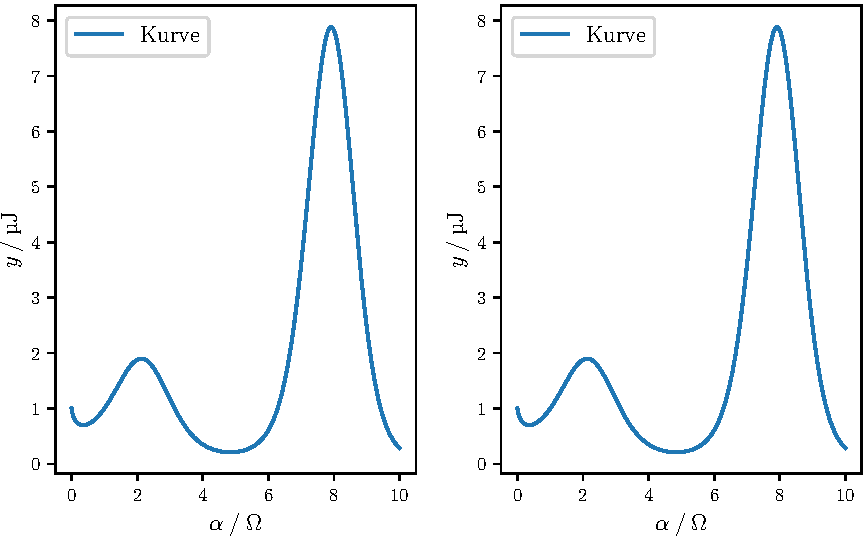
\includegraphics{plot.pdf}
  \caption{Plot.}
  \label{fig:plot}
\end{figure}
